\documentclass[11pt]{ctexart}

\usepackage{multicol}
%\usepackage{mwe}
\usepackage{subfigure}
\usepackage{mathtools}
\usepackage{graphicx}
\usepackage{amsmath}
\usepackage{mathrsfs}
\usepackage[top=0.5in,bottom=1in,left=1in,right=1in]{geometry}
\usepackage{pdflscape}
\usepackage{times}
\usepackage{bm}
%\usepackage{setspace}
\usepackage{color}
\usepackage{caption}
\usepackage{amsmath}
\usepackage{amssymb}
\usepackage{CJK}
\usepackage{longtable}
%\usepackage[final]{pdfpages}
\usepackage{listings}
\usepackage{textcomp}
\usepackage{xcolor}
\usepackage{algorithm2e}
\usepackage{float}
\usepackage{algorithmicx}
\usepackage{algpseudocode}
\usepackage{hyperref}

\hypersetup{hidelinks,
	colorlinks=true,
	allcolors=black,
	pdfstartview=Fit,
	breaklinks=true}

\pagestyle{plain}




\begin{document}

\title{第十一周实习报告20220520}
\author{宋欣源}
\date{\today}

\maketitle % need full-width title

\CTEXsetup[format={\Large\bfseries}]{section}

\section{第一,综述}

下面对于这些天实习的工作做一个报告。现在就两周的工作做一个总结
我这周主要在raw3数据集上进行。首先是解决了高CPU占有率的问题,然后对于convolutedRNN进行了改进,最后研究创新了新的CNN模型

\section{第二,CPU问题}
这几天对于这个问题进行了大量实验,从几个角度入手进行解决。首先,对于不同的模型,都进行了实验,发现,不仅仅是我自己写的RNN模型,还是torch.nn的RNN模快,还是我自己实现的fold加unfold的CNN模型,还是torch.nn自带的CNN模块,都有CPU高占用率的问题。CPU占用普遍在2000\%以上,近百个逻辑核心全部占满。说明主要原因应该不是我的代码的问题。因此查找了有关内容,找到了如下解释:

Xeon CPU gold系列采用avx-512指令集,而一般的CPU采用avx-2指令集,新的指令集容易造成CPU占用率过高。avx-512采用逻辑分配的方式,将任务分配给尽可能多的逻辑单元,保证在 \par CPU端的运行效率最高。因此如果不限制CPU核心数目,有如下差别:

\begin{figure}[H]
\begin{center}
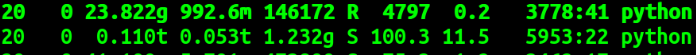
\includegraphics[width=0.8\textwidth]{1.PNG}
\end{center}
\caption{CPU performance top}
\label{FIG.1}
\end{figure}
服务器96个核心,在三层CNN网络这一简单任务,在linux端限制核心数目和不限制核心数目的区别,不限制情况况下CPU利用率4797,整体CPU利用率4797/9600约50\%,采用GPU进行训练。在运行时间上,全开96核心所需要的时间为4.83秒,服务器频率达到2.3Ghz。而只开一个cpu所用的时间为5.22秒,GPU频率达到2.4Ghz。经过查阅Xeon CPU相关文档,发现Xeon CPU的指令集架构有保护作用,对num\_works进行良好分配,导致Xeon CPU不至于达到工作频率的90\%以上,起到保护的目的。同时,通过资源分配,使CPU能够最快速度的完成任务。

但是,最快速度的提升只有很少一点,经过多次实验,num\_works设置成1和96的情况下,由于是GPU训练,区别不大,经过psutil输出CPU状态,大部分CPU实质上处于等待状态,没有参与实质的运算。但是IO可能占用,还有就是CPU给GPU做调度。因此体现出高占有率的特性。对于一致内存的服务器,完全可以不开所有核心,在进行GPU训练的同时使用CPU进行其他工作。对于个人电脑,或者太湖之光,华为升腾之类的非一致内存服务器,整个服务器只能同时运行一个进程,占满CPU就不能做别的了。而且对于4.6Ghz的Xeon gold系列CPU,保护作用具体处于2.3Ghz还是2.4Ghz区别不大。因此完全没必要全开96个核心。只需要设置成1就好。

在这一点上,torch也有同样的功能,torch.set\_num\_works(1),torch.set\_num\_threads(1)利用这两个命令将CPU的核心数和线程数控制在1。经过查阅torch文档,这两个会互相作用,因此最好都设置成1。在torch文档内,这两个指令也是通过调用Linux指令完成的。和我原来的做法没有区别。进过多次实验,确实没区别。因此多核心的解决办法就是设置torch.set\_num\_threads(1)。经过设置,核心控制在1,单个程序CPU占用有率最高100\%。而且进行了大量实验,发现训练的速度,训练的结果和设置前没有显著区别,全开的时候10min一个epoche,开一个大约需要12min。

那么RNN base和我实现的RNN base有没有造成CPU的更高占用呢,并没有。我之前观察到在运行的时候CPU有提升,可能是随机涨落的结果。经过反复实验,也没有出现一定导致结果的情况。对于在RNN里init hidden\_state的结果,也没有一定导致CPU使用上升。同时,不论init采用的是device = conv.weight还是.cuda()最后结果是完全一样的。因此上次说的这个点也不是最后的原因。


\section{第三、convolutedRNN}
\subsection{综述}
之前研究了RNN的框架,现在解决了框架造成CPU占用过高的问题,经过上次的讨论,打算对convolutedRNN进行修改,交换层与层的结构,加入avgpool,batchnorm,relu或者其他自定层。由于在CNN上,这些层往往使用非常多次,很难有什么idea能一部达到效果,因此在convolutedRNN \par上线进行试验。convolutedRNN采用的是学习截面的方法,卷积层较少,同时卷积层大小也较小,可以进行有效的实验。之前基于convolutedRNN的研究最后找到了几个最后效果比较好的模型进行保留,在这几个上进行实验。同时也要考虑每个模型的数学表达式,防止出现梯度消失和梯度爆炸的情况。

\subsection{convGRU}
上次对于convGRU认识到。两个都用kernel\_size = 3卷积层效果较好,在raw3上能到到pnl2.6的结果因此基于这个模型进行修正。对于效果第二好的两次kernel\_size = 1再用两次kernel\_size = 3进行尝试一部分

同时,删掉了pointwise层,只保留一个线性层,对于元模型来说有不小的影响,但是在这个个基础上继续做力求提高

模型1(原模型):convGRU(conv+conv)\_2layer(layer1(batch:1,kernel:3), layer2(batch:1,kernel:3)) 替换第一个线性层为卷积

模型原表现(只保留最后一个线性层,原模型最高2.6去掉后2.5)
{\kaishu \small IC: 0.067, pnl:2.49}

~\\
模型2:convGRU(conv\_avg+conv\_avg)\_2layer(layer1(batch:1,kernel:3), layer2(batch:1,kernel:3))

模型表现{\kaishu \small IC: 0.064, pnl:2.39}

~\\
模型3:convGRU(conv\_avg\_relu+conv\_avg+relu)\_2layer(layer1(batch:1,kernel:3), 

layer2(batch:1,kernel:3))

模型表现{\kaishu \small IC: 0.062, pnl:2.35}


~\\
模型4:convGRU(avg\_conv\_batchnorm+avg\_conv\_batchnorm)

\_2layer(layer1(batch:1,kernel:3), layer2(batch:1,kernel:3))

模型表现{\kaishu \small IC: 0.064, pnl:2.41}

~\\
模型5:convGRU(conv\_avg\_batchnorm+conv\_avg)

\_2layer(layer1(batch:1,kernel:3), layer2(batch:1,kernel:3))

模型表现{\kaishu \small IC: 0.068, pnl:2.55}

模型有了显著提高,沿着这个方向继续,从数据流的角度出发,batchnorm在两个conv中间其效果,在最后一个conv特征提取层会降低效果,原因大概是会让下一个conv的提取更加优美更加均匀。因此一定要先avg再conv再batchnorm下一次直接采用conv

~\\
模型6:convGRU(avg\_conv\_batchnorm+conv\_relu)

\_2layer(layer1(batch:1,kernel:3), layer2(batch:1,kernel:3))

模型表现{\kaishu \small IC: 0.071, pnl:2.69}

效果果然强于之前的模型,看来在曾细节上有很大讲究,那么对于relu的模型,应该怎么加呢,进行对比和消融实验

~\\
模型7:convGRU(avg\_conv\_batchnorm+conv\_avg\_relu)

\_2layer(layer1(batch:1,kernel:3), layer2(batch:1,kernel:3))

模型表现{\kaishu \small IC: 0.066, pnl:2.59}

~\\
模型8:convGRU(avg\_conv\_relu\_batchnorm+conv\_avg)

\_2layer(layer1(batch:1,kernel:3), layer2(batch:1,kernel:3))

模型表现{\kaishu \small IC: 0.067, pnl:2.44}

模型表现都一般,看样子不能加relu,又进行了很多类似的尝试,结果不见得很好。不妨换一种思路,多加avgpool层,让提取的结果更善,体现出外势的结果。从信息流的角度,让信息再截面上更加均匀,不会导致某一个数据对截面的演化效果贡献很大。

~\\
模型9:
convGRU(avg\_conv\_avg\_avg\_batchnorm+avg\_conv\_avg\_avg)

\_2layer(layer1(batch:1,kernel:3), layer2(batch:1,kernel:3))

模型表现{\kaishu \small IC: 0.068, pnl:2.49}

~\\
模型10:
convGRU(avg\_conv\_avg\_avg\_batchnorm\_relu+avg\_conv

\_batchnorm\_avg)\_2layer(layer1(batch:1,kernel:3), layer2(batch:1,kernel:3))

模型表现{\kaishu \small IC: 0.072, pnl:2.59}

可以看到模型表现又开始提高,那么继续增加avg,同时在avg之间加入relu

~\\
模型11:
convGRU(avg\_conv\_avg\_relu\_avg\_batchnorm\_relu+

avg\_conv\_batchnorm\_relu\_avg)\_2layer(layer1(batch:1,kernel:3), 

layer2(batch:1,kernel:3))

模型表现{\kaishu \small IC: 0.069, pnl:2.64}

~\\
模型12:
convGRU(avg\_conv\_avg\_relu\_avg\_batchnorm+

avg\_conv\_avg\_relu\_avg)\_2layer(layer1(batch:1,kernel:3), 

layer2(batch:1,kernel:3))

模型表现{\kaishu \small IC: 0.077, pnl:2.73}

只用了两层CNN,模型过拟合现象不明显,往往需要跑40个epoche以上才到好的效果,因此暂时不加入dropout情况。加入之后进行尝试,发现效果变差,而且运行需要的时间非常非常长。不建议这么做,想别的方向

目前到达2.73,效果已经不断提高。但是交换各类的层的办法已经都尝试了,因此尝试另一种效果比较好的GRU网络,四层GRU。首先先用kernel\_size = 1的卷积层进行提取两层,再用两次kernel\_size = 3的卷积层进行提取。

~\\
模型13(原模型):convGRU(conv+conv+conv+conv)\_4layer

(layer1(batch:n,kernel:1),layer2(batch:n,kernel:1),

layer3(batch:1,kernel:3),layer4(batch:1,kernel:3)) 替换第一个线性层为卷积

模型原表现(只保留最后一个线性层,原模型最高2.6去掉后2.2)

{\kaishu \small IC: 0.046, pnl:2.25}

~\\
模型14:convGRU(avg\_conv\_avg\_relu\_avg\_batchnorm+

avg\_conv\_avg\_relu\_avg+avg\_conv\_avg\_relu\_avg+

avg\_conv\_avg\_relu\_avg)\_4layer(layer1(batch:n,kernel:1), 

layer2(batch:n,kernel:1),layer3(batch:1,kernel:3),

layer4(batch:1,kernel:3))

根据上面的经验进行修改,有了显著提高

模型表现{\kaishu \small IC: 0.068, pnl:2.55}

~\\
模型15:convGRU(avg\_conv\_avg\_relu\_avg\_batchnorm+

avg\_conv\_avg\_relu\_avg\_batchnorm+

avg\_conv\_avg\_relu\_avg\_batchnorm+

avg\_conv\_avg\_relu\_avg)\_4layer(layer1(batch:n,kernel:1), 

layer2(batch:n,kernel:1),layer3(batch:1,kernel:3),layer4(batch:1,kernel:3))

继续沿用batchnorm的结果,又有提高

模型表现{\kaishu \small IC: 0.069, pnl:2.58}

~\\
模型16:convGRU(avg\_conv\_avg\_relu\_avg\_batchnorm+

avg\_conv\_avg\_avg\_batchnorm+

avg\_conv\_avg\_avg\_batchnorm+

avg\_conv\_avg\_relu\_avg)\_4layer(layer1(batch:n,kernel:1), 

layer2(batch:n,kernel:1),layer3(batch:1,kernel:3),layer4(batch:1,kernel:3))

对relu进行抛弃,多层relu对结果有影响,模型又有提高

模型表现{\kaishu \small IC: 0.072, pnl:2.63}

~\\
模型17:convGRU(avg\_conv\_avg\_relu\_avg\_batchnorm+

avg\_conv\_batchnorm+

avg\_conv\_batchnorm+

avg\_conv\_avg\_relu\_avg)\_4layer

(layer1(batch:n,kernel:1),layer2(batch:n,kernel:1),

layer3(batch:1,kernel:3),layer4(batch:1,kernel:3))

清除大量的avg层,层数太多可能造成模型整体偏移。

模型表现{\kaishu \small IC: 0.069, pnl:2.64}


~\\
模型18:convGRU(avg\_conv\_avg\_relu\_avg\_batchnorm+

avg\_conv\_batchnorm+

avg\_conv\_batchnorm+

avg\_conv\_avg\_relu\_avg)\_4layer(layer1(batch:n,kernel:1), 

layer2(batch:n,kernel:1),layer3(batch:1,kernel:3),layer4(batch:1,kernel:3))

对于上面的思路,很难有大的进步,相关内容也进行了尝试,在保证梯度不爆炸的前提下,其他模型也没有这些效果好。因此不再赘述。那么只能进行方向跳跃,加大步伐。看看能不能找到更好的结果。

模型表现{\kaishu \small IC: 0.069, pnl:2.64}

~\\
模型19:convGRU(avg\_conv\_batchnorm+conv\_batchnorm+

conv\_batchnorm+avg\_conv\_avg\_relu\_avg)\_4layer

(layer1(batch:n,kernel:1), 

layer2(batch:n,kernel:1),

layer3(batch:1,kernel:3),layer4(batch:1,kernel:3))

在模型19中对于中间层的convolution,以提取信息为主,而两侧的convolution以准备数据为主,依靠这个思路,最后的的conv卷积层需要尽可能地avg和batchnorm,保证结果,第一层的conv卷积层,要将数据准备到合理的地步,加入一个avg和一个batchnorm。中间的卷积层,则需要加入 \par batchnorm保证结果不偏移,但是对于relu和avgpool要越少越好。
根据上面的经验进行修改,有了显著提高

模型表现{\kaishu \small IC: 0.078, pnl:2.74}

~\\
模型20:convGRU(avg\_avg\_conv\_batchnorm+conv\_batchnorm+

conv\_batchnorm+conv\_avg\_avg\_relu\_avg)

\_4layer(layer1(batch:n,kernel:1), 

layer2(batch:n,kernel:1),layer3(batch:1,kernel:3),

layer4(batch:1,kernel:3))

得到了初步胜利,模型19在上面的基础上,不妨取消不该出现的avg,在关键地方进行多加.这样做的思路就是先把数据提高到合适的地步,再采用合适的conv进行提取,提取的时候只采用 \par batchnorm保证数据的连贯性和信息的均匀。最后再采用多次avg将特征放到平面上。这种做法采用的卷积核是(1,1,3,3)的结构,似乎并不适用这个结构,因为前两次使用1的卷积核但是对于信息的处理功能不同。后两次采用3的卷积核后两次功能也不同,(1,1,3,3)是之前发现的较好的模型,并不一定适合现在的结构。不妨采用(1,3,3,1)的结构进行研究。

模型表现{\kaishu \small IC: 0.076, pnl:2.754}

~\\
模型21:convGRU(avg\_avg\_conv\_batchnorm+

conv\_batchnorm+

conv\_batchnorm+
conv\_avg\_avg\_relu\_avg)\_4layer

(layer1(batch:n,kernel:1), layer2(batch:·,kernel:3),layer3(batch:1,kernel:3),

layer4(batch:n,kernel:1))

在这个模型中,出现了数据过拟合,在第四个epoche开始变差,因此加入dropout进行调节

模型表现{\kaishu \small IC: 0.073, pnl:2.74}

~\\
模型22:convGRU(avg\_avg\_conv\_batchnorm+

conv\_batchnorm+

conv\_batchnorm+

conv\_avg\_avg\_dropout\_relu\_avg)\_4layer

(layer1(batch:n,kernel:1), 

layer2(batch:·,kernel:3),layer3(batch:1,kernel:3),layer4(batch:n,kernel:1))

在模型22中,解决了过拟合问题,最后结果也没有提高,大概15个epoche开始过拟合。

模型表现{\kaishu \small IC: 0.072, pnl:2.71}

~\\
模型23:convGRU(avg\_conv\_batchnorm+conv\_batchnorm+

conv\_batchnorm\_dropout+conv\_avg\_relu)\_4layer

(layer1(batch:n,kernel:1), 

layer2(batch:·,kernel:3),layer3(batch:1,kernel:3),

layer4(batch:n,kernel:1))

在模型23中,感觉模型比较冗余,于是进行了大量修改,删去了不合适的avg,同时找到了 \par dropout的最佳位置。并不是放在最后而是放在中间.由此可见,对于不同的模型,dropout的位置也有讲究.因此效果进一步提高。接下来的尝试,效果又差不多,也就不再赘述了,因此我决定再次跳跃。既然这个结构是先准备数据,然后提取特征,再将特征完美的洗好,而且从dropout上,也是对于提取的特征进行dropout。很容易想到利用CV里的常用结构,也是之前再CNN1d中证明有效的bottleneck结构进行改写。同时,目前最有效地结构是kernel\_size为(1,3,3,1)的结果,很容易想到 \par bottleneck的kernel\_size是(1,3,1)。从这三个角度,似乎bottleneck的模式最适合再 \par ConvolutedRNN中当作CNN进行特征提取。

模型表现{\kaishu \small IC: 0.075, pnl:2.76}


~\\
模型24:convGRU(conv(1,256)\_batchnorm+

conv(3,256)\_batchnorm\_dropout+conv(1,256)

\_avg\_relu)\_3layer(layer1(batch:n,kernel:1), 

layer2(batch:·,kernel:3),layer4(batch:n,kernel:1))

在模型24中,采用bottleneck的格式,按照上面的经验,采取3层CNN作为RNN的特征提取,其中kernel\_size为(1,3,1)。同时,按照上面的经验,在最合理的位置上添加了avg和relu。提取特征维度都是256,没有采用其他维度。事实证明256也是最适合这个模型的。(长期经验来看,raw5数据更适合64,可以简单理解为正好12是3的4倍。)模型效果有了显著提高。

模型表现{\kaishu \small IC: 0.079, pnl:2.79}

~\\
模型25:convGRU(conv(1,256)\_batchnorm+

conv(3,256)\_batchnorm\_dropout+conv(1,256)

\_avg\_relu)\_3layer(layer1(batch:n,kernel:1),

 layer2(batch:·,kernel:3),layer4(batch:n,kernel:1))

在模型25中,由于之前阅读了整个pytorch文档,得知nn.dropout还有一个替身叫 \par nn.featuredropout,这个替身专门将整个特征进行擦除,而不是将数据中的值随机擦除。显然更适合现在的情况,将中间层提取的特征直接进行随机擦除,但是必须保证擦除数量足够少,因此p = 0.9,进行修改以后,最后的结果更优,达到了2.83。这个结果是目前最好的,但是pnl long不够高,之前有的模型long比较好。以后对pnl long进行更过关注

模型表现{\kaishu \small IC: 0.081, pnl:2.83}

模型25是在convGRUcell里实验出的表现最好的模型。这个办法目前证明有效,但是还需要大量实验提高认知。

\begin{figure}[H]

\begin{center}
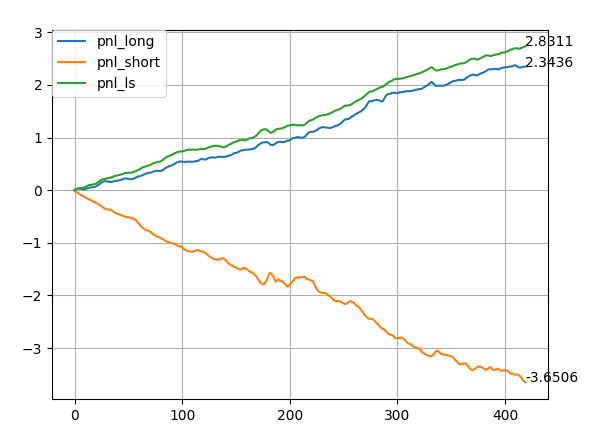
\includegraphics[width=0.8\textwidth]{3.PNG}
\end{center}
\caption{bottleneck convGRU best pnl figure}
\label{FIG.2}
\end{figure}


\subsection{convLSTM}
对于convLSTM的意义在于,根据LSTM的公式,需要做一次线性层,那么可以将线性层替换成卷积层convolution.结构和最基础的结构一样。那么对这一次线性层进行改造。LSTM的效果本身也比较好,但是在这个结构上,可操作空间就大大减少了,只有一个线性层,所以在线性层上进行了各种实验。

模型原表现(只保留最后一个线性层,原模型最高2.6,去掉后2.3)

模型1:convLSTM(conv)\_2layer(layer1(batch:1,kernel:3), layer2(batch:1,kernel:3))

模型表现{\kaishu \small IC: 0.055, pnl:2.3}

~\\
模型2:convLSTM(avg\_conv)\_2layer

(layer1(batch:1,kernel:3), layer2(batch:1,kernel:3))

按照上面的经验

模型表现{\kaishu \small IC: 0.053, pnl:2.4}

~\\
模型3:convLSTM(avg\_conv\_batchnorm)

模型表现\_2layer(layer1(batch:1,kernel:3), layer2(batch:1,kernel:3))

{\kaishu \small IC: 0.049, pnl:2.5}

~\\
模型4:convLSTM(avg\_conv\_avg\_relu\_avg)

\_2layer(layer1(batch:1,kernel:3), layer2(batch:1,kernel:3))

按照上面总结的经验,可以用这个办法。

模型表现{\kaishu \small IC: 0.068, pnl:2.65}

~\\
模型5:convLSTM(avg\_avg\_conv\_avg\_avg\_relu\_avg)

\_2layer(layer1(batch:1,kernel:3), layer2(batch:1,kernel:3))

同样道理可以叠加avg

模型表现{\kaishu \small IC: 0.067, pnl:2.64}

~\\
模型6:convLSTM(avg\_conv\_avg\_dropout\_batchnorm\_relu)

\_2layer(layer1(batch:1,kernel:3), layer2(batch:1,kernel:3))

同样道理可以加入batchnorm和dropout

模型表现{\kaishu \small IC: 0.071, pnl:2.7}

~\\
模型7:convLSTM(conv\_avg\_batchnorm\_avg\_relu)

\_2layer(layer1(batch:1,kernel:3), layer2(batch:1,kernel:3))

精简模型

模型表现{\kaishu \small IC: 0.075, pnl:2.74}

在这里说明一下,如果采用kernel\_size = 1的结果,那么和poitwise没啥区别,所以直接舍弃了,目前就是要在没有pointwise的基础上进行试验。LSTM普遍没有GRU效果好,肯定是卷积层数越多越好,但是层数到4以后,效果又会变差,所以最佳效果是3层。同时LSTM的操作空间远远小于GRU,对于GRU还有大量的实验空间和跳跃方向,。但是LSTM方向较少。LSTM也可以改写成有很多层的形式,但是那样就是纯属人为搞得复杂,其结果很不善。在信息流上也不自然。所以就不尝试了。另外LSTMcell在RNN中很容易梯度爆炸,门越多,需要考虑的计算层数越多,也不方便加入更多的CNN操作。整体上看,有进行了很多实验,大多以梯度爆炸或者梯度消失而失败。所以这个cell比GRUcell整体结果上要差。

模型7是在convLSTMcell里实验出的表现最好的模型。

\begin{figure}[H]

\begin{center}
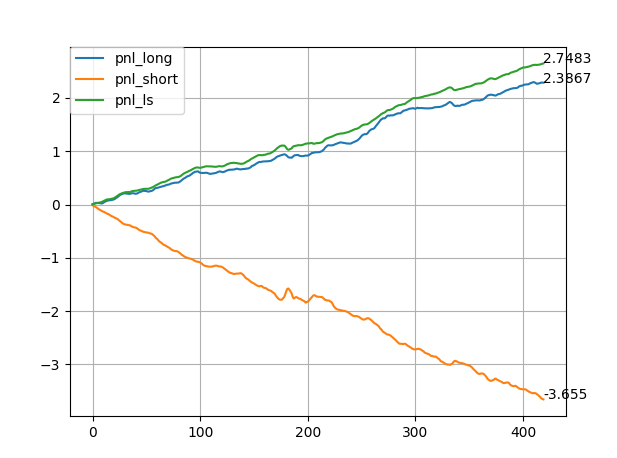
\includegraphics[width=0.8\textwidth]{2.PNG}
\end{center}
\caption{one CNN convLSTM best pnl figure}
\label{FIG.3}
\end{figure}


\subsection{改进思路}
\begin{itemize}
  \item [0)]
    这一部分研究属于采用老师推荐的办法对ConvolutedRNN进行细致研究。首先CRNN上不适合采用特别复杂的CNN结构。事实证明4层效果开始显著变差,所以目前采用的是3层 \par bottleneck效果最好。兼顾计算量,过拟合,效果和特征提取。所以在这仅有的三层上,可以改编层的关系,细致研究。目前还有很多可以实验的办法,比如采用bottleneck2结构,或者mobilenet结构,都是层数很低的cnn网络。可以在RNN上替换线性层进行试验。由于解决了CPU占有率高的问题,但是并没有造成计算时间的显著增加,因此还有很多可操作余地。
  \item [1)]
    另一个改造的效果就是细致的研究CNN的提取。比如stride,dilation,groups等参数,在这个场景下如何细致的影响CRNN的最后结果。这些细致的改变最后造成的影响是非常大的。比如可以采用之前研究的多种dilation叠加的办法,多种stride叠加的办法,增强cNN的感受野。
  \item [2)]
    我经验大量实验,已经证明采用数据增强的办法(就是数据合并成不同的维度多次输入模型最后相加)这个办法结果不好。所以也没有在文中将结果列出来。这个办法在raw5数据上表现较好,在raw3上没有这个必要,这和数据的逻辑有关。raw5和最终的y15 labels之间有本身关系不密切,需要多种观点的数据进行叠加找到其中的关系,但是raw3本身关系密切,在时间序列上进行多种输入似乎意义不大。
  \item [3)]
    第四,抛弃了最后的linear和pointwise,起初模型是有效果变差,但是通过努力一点一点效果提高起来。
  \item [4)]
    最后,我觉得CRNN就告一段落,之前采用的调整层的办法,对于CNN积累了很多经验,按照这个办法在CNN上进行尝试,肯定有较好的提升。
\end{itemize}

\section{第四,CNN1d}

这段时间的CNN1d没有像上面的结果一样从层的堆叠和意义以及信息流的角度进行设计,而是从CNN1d的角度重新开始卷积层和特征提取。不再基于某个backbone而是进行自己的研究。

\subsection{模型和表现}

首先类似于之前研究的deeplab模型,我们至少要从多个卷积层开始。最基础的模型是3层 \par featuremap卷积网。采用5的卷积核三层convolution网络作为基底。同时尝试普通cnn和stride = kernel\_size两个方向。

模型1:普通CNN1d(CNN1d(5,1)*3+linear)

模型表现{\kaishu \small IC: 0.043, pnl:2.4}

~\\
模型2:普通CNN1d(CNN1d(5,1)*3+CNN1d(3,1)*2+linear)

在此基础上,加入两个新的卷积层,其他保持不变

模型表现{\kaishu \small IC: 0.048, pnl:2.5}


~\\
模型3:普通CNN1d(CNN1d(5,1)*3+CNN1d(3,1)+down\_sample(3,1)+linear)

采用down\_sample的办法将维度降低到512维

模型表现{\kaishu \small IC: 0.044, pnl:2.4}


~\\
模型4:普通CNN1d(CNN1d(5,1)*3+CNN1d(3,1)+

down\_sample(3,1)+down\_sample(3,1)+linear)

采用down\_sample的办法将维度降低到256维,经过降维,运算更加稳定,结果更加稳定

模型表现{\kaishu \small IC: 0.046, pnl:2.5}

~\\
模型5:普通CNN1d(CNN1d(5,1)*3+CNN1d(3,1)+

down\_sample(3,1)+down\_sample(3,1)+ CNN1d(3,1)+linear)

采用down\_sample的办法将维度降低到256维,经过降维,运算更加稳定,结果更加稳定,效果又一点提高

模型表现{\kaishu \small IC: 0.052, pnl:2.6}

~\\
模型6:
普通CNN1d(CNN1d(5,1)*3+CNN1d(3,2)+CNN1d(1,1)+linear)

经过上面的研究。我们开始调整步距来提高效果。因为最后放弃了pointwise在时间上的观点,所以开始进行调整。
首先还是基于模型1的结果,对于模型2,可以修改为这个模型。利用  \par CNN1d(3)调整步距,然后接两个kernel\_size为1的层。实现了降低序列长度和提高特征维度。结果和原有模型不相上下。

模型表现{\kaishu \small IC: 0.054, pnl:2.62}

~\\
模型7:普通CNN1d(CNN1d(5,1)*3+CNN1d(3,2)+CNN1d(1,1)*2+

CNN1d(3,2)+CNN1d(1,1)*2+linear)

经过上面的研究。我们再次调整步距来提高效果。由于不能单纯的增加,所以仍然采用这个办法。

模型表现{\kaishu \small IC: 0.055, pnl:2.64}


~\\
模型8:普通CNN1d(CNN1d(5,1)*3+CNN1d(3,2)+CNN1d(1,1)*2+

CNN1d(3,2)+CNN1d(1,1)*2+down\_sample(CNN1d(3,2)+CNN1d(1,1))+linear)

对于downsample,也采用同样的办法

模型表现{\kaishu \small IC: 0.057, pnl:2.58}


~\\
模型9:普通CNN1d(CNN1d(5,1)*3+CNN1d(3,2)+CNN1d(1,1)*2+

CNN1d(3,2)+CNN1d(1,1)*2+down\_sample(CNN1d(3,2)+CNN1d(1,1)*3)+

down\_sample(CNN1d(3,2)+CNN1d(1,1)*3)+linear)

对于downsample,也采用同样的办法.IC继续上升,但是pnl已经不变。

模型表现{\kaishu \small IC: 0.059, pnl:2.60}


~\\
模型9:普通CNN1d(CNN1d(5,1)*3+CNN1d(3,2)+CNN1d(1,1)*2+

CNN1d(3,2)+CNN1d(1,1)*2+down\_sample(CNN1d(3,2)+CNN1d(1,1)*3)+

down\_sample(CNN1d(3,2)+CNN1d(1,1)*3)+avgpool+CNN1(1,1)+relu+linear)

最后经过avgpool和CNN1d(1,1)达到目的,这时候时间序列已经尺缩到1。效果有了明显好转。但还需要尝试。
这里我讲一下为什么要这么做。首先通过特征提取,当维度升高到512以后,不适合再生高纬度,所以采用down\_sample的办法降低维度。让最后维度落在256.第二。在尺度方面,每次都用stride = 2来提取,让每次长度变为之前的一半。
尺缩的另一个办法是利用avgpool。不妨将上述几个模型的尺缩换成avgpool的缩进,

模型表现{\kaishu \small IC: 0.066, pnl:2.7}

~\\
模型10:普通CNN1d(CNN1d(5,1)*3+(avg+CNN1d(3,1)+CNN1d(1,1)*1)+

(avg+CNN1d(3,2)+CNN1d(1,1)*1)+down\_sample(avg+CNN1d(3,2)+CNN1d(1,1)*2)+

down\_sample(avg+CNN1d(3,2)+CNN1d(1,1)*2)+avgpool+CNN1(1,1)+relu+linear)

首先尝试将所有的全换成avgpool,效果有所下降,这时候效果不是太好,而且经常出现不收敛的结果。首先加上relu

模型表现{\kaishu \small IC: 0.044, pnl:2.4}

~\\
模型11:普通CNN1d(CNN1d(5,1)*3+relu+(avg+CNN1d(3,2)+CNN1d(1,1)*1+relu)+

(avg+CNN1d(3,2)+CNN1d(1,1)*1+relu)+down\_sample(CNN1d(3,2)+CNN1d(1,1)*3+relu)+

down\_sample(CNN1d(3,2)+CNN1d(1,1)*3+relu)+avgpool+CNN1(1,1)+relu+linear)

效果依然不理想,那么把其中一部分avg还用stride来实现。具体上,对于down\_sample而言,本身就是让维度降低,如果其中加入了avg,最后模型经常学不到东西。事实也是如此。维度降低以后信息更加集中,再采用avg让信息流失严重。因此从down\_sample开始全都采用stride = 2。结果是找回了原有表现。那么avg到底有没有用呢,首先让运行结果更加稳定,每次都能跑出类似的结果。其次avg的位置还有待讲究,可以有更多提高的空间

模型表现{\kaishu \small IC: 0.068, pnl:2.73}

对于这个模型的骨架,画图如下:
\begin{figure}[H]

\begin{center}
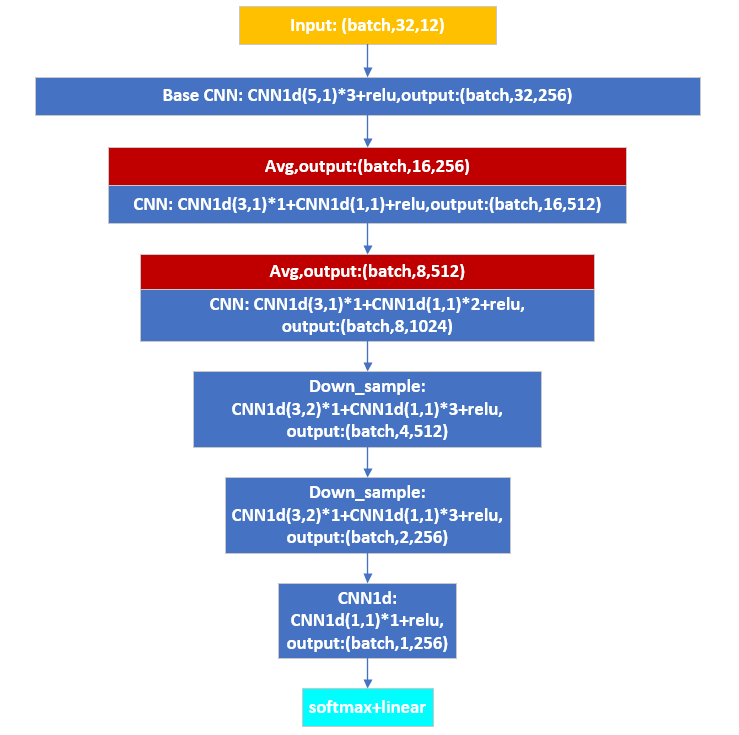
\includegraphics[width=1.0\textwidth]{4.PNG}
\end{center}
\caption{CNN1d骨架}
\label{FIG.4}
\end{figure}

表现如下:
\begin{figure}[H]

\begin{center}
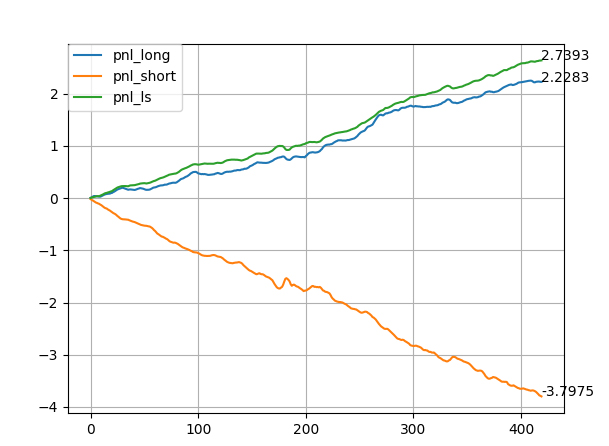
\includegraphics[width=0.8\textwidth]{5.PNG}
\end{center}
\caption{CNN1d pnl fugure}
\label{FIG.5}
\end{figure}


~\\
模型12:普通CNN1d(CNN1d(5,1)*3+relu+(avg+CNN1d(3,2)+relu+CNN1d(1,1)*1)+

(avg+CNN1d(3,2)+relu+CNN1d(1,1)*1)+down\_sample(CNN1d(3,2)+relu+CNN1d(1,1)*3)+

down\_sample(CNN1d(3,2)+relu+CNN1d(1,1)*3)+avgpool+CNN1(1,1)+relu+linear)

将relu的位置进行修改尝试,结果有所下滑

模型表现{\kaishu \small IC: 0.064, pnl:2.6}

~\\
模型13:普通CNN1d(CNN1d(5,1)*3+relu+(avg+CNN1d(3,2)+CNN1d(1,1)*1+batchnorm+relu)+

(avg+CNN1d(3,2)+CNN1d(1,1)*1+batchnorm+relu)+

down\_sample(CNN1d(3,2)+CNN1d(1,1)*3+batchnorm+relu)+

down\_sample(CNN1d(3,2)+CNN1d(1,1)*3+batchnorm+relu)+

avgpool+CNN1(1,1)+relu+linear)

加入了batchnorm,效果有所下滑

模型表现{\kaishu \small IC: 0.062, pnl:2.5}

\subsection{改进思路}
\begin{itemize}
  \item [0)]
  第一就是继续研究avg,relu,batchnorm,max的位置,或者模型的骨架结构。
  \item [1)]
  模型最后的衔接,除了这种模式,还有其他的模式,在不适用pointwise和linear之后,模型最后接上最后于1层linear还有待研究
  \item [2)]
  调整dialtion,groups参数,用不同的观点进行卷积。
\end{itemize}


\section{第五、总结}
\begin{itemize}
  \item [1)]
  这一周多一点,时间比较紧张,加上在家办公,效率较低,又解决了CPU占用率的问题,对于这两个角度还需要深入研究。从下周开始,方向就选CNN1d模型,开始不依赖传统的 \par backbone利用自己的经验开始搭建,找表现较好的方向。同时经常进行跳跃,除了找到局部最优解,还要注重外势的研究。
  \item [2)]
  第二,对于convolutedRNN模型,进行了相当细致的研究。接下来准备再CNN的参数上下功夫,在已有的优秀模型上进一步细致调整。这些调整看似很细小,其实最后的结果经常大相径庭。还要从信息流和数据的角度给予评价和理解。
  \item [3)]
  第三,对于CNN1d系列,下周就继续搭建自己的backbone。尝试avg的不同位置,relu的不同位置,加入batchnorm,利用已经积累的CRNN调整的经验进行搭建。同时如果发现附近的结果表现提高都有限。就进行跳跃。迈一大步看看别的情况。
\end{itemize}


\end{document} 